
\paragraph{4. Do new relations introduce new observable behaviors?}
    In any candidate execution, reordering events $e$ and $d$ eliminates the relation $\reln{e}{hb}{d}$ and introduces the new relation $\reln{d}{hb}{e}$.
    This new relation itself could introduce new observable behaviors.  
    Hence, let us first consider the variants of events $e$ and $d$ that we need to analyze from the previous table:
    \begin{tasks}(2)
        \task $\event{e}{R} \ \wedge \ \event{d}{R} \ \wedge \et{e}{uo} \ \wedge \et{d}{uo}$
        \task $\event{e}{R} \ \wedge \ \event{d}{R} \ \wedge \et{e}{uo} \ \wedge \et{d}{sc}$
        \task $\event{e}{R} \ \wedge \ \event{d}{W} \ \wedge \et{e}{uo} \ \wedge \et{d}{uo}$
        \task $\event{e}{W} \ \wedge \ \event{d}{R} \ \wedge \et{e}{uo} \ \wedge \et{d}{uo}$
        \task $\event{e}{W} \ \wedge \ \event{d}{R} \ \wedge \et{e}{uo} \ \wedge \et{d}{sc}$
        \task $\event{e}{W} \ \wedge \ \event{d}{R} \ \wedge \et{e}{sc} \ \wedge \et{d}{uo}$
        \task $\event{e}{W} \ \wedge \ \event{d}{W} \ \wedge \et{e}{uo} \ \wedge \et{d}{uo}$
        \task $\event{e}{W} \ \wedge \ \event{d}{W} \ \wedge \et{e}{sc} \ \wedge \et{d}{uo}$
    \end{tasks}

    We analyze each of the above case one by one by first considering the original relation ($\reln{e}{hb}{d}$) and the reordered one ($\reln{d}{hb}{e}$). 
    \begin{itemize}
        \item (a) and (b) do not fit any pattern of our Axioms, hence even after reordering the agent order between them does not match any other axiom. Hence this relation does not introduce any new observable behavior. This is irrespective of the range between the two read events.
        \item (c) fits in the pattern of Axiom \ref{CoRe}, when they have at least overlapping ranges. Before reordering, $d$ is not allowed to read from $e$, but after reordering, it can. Hence this relation can introduce observable behavior if the range between events $e$ and $d$ at least overlap. 
        \item (d), (e) and (f) can fit in the pattern of Axioms \ref{CoRe} and \ref{SeqCsAt}, if $e$ and $d$ at least have overlapping ranges, preventing $d$ from reading parts of $e$ or some parts of another write $k$ due to $e$ being the intervening write. But after reordering, $d$ is allowed to read parts of $k$, which introduces new observable behaviors.
        \item (g) and (h) can fit in the pattern of Axioms \ref{CoRe} and \ref{SeqCsAt}, if they have at least overlapping ranges. Before reordering, the agent order between $e$ and $d$ could prevent some read $k$ from reading parts of $e$. This is not the case after reordering, thus possibly introducing a new observable behavior. 
    \end{itemize}

    In summary, on inferring the role on the Axioms on the relation between $e$ and $d$, notice that if both $e$ and $d$ are read events then the range does not matter. For all other cases, if events $e$ and $d$ have at least overlapping ranges, one could introduce a new observable behavior after reordering them.
    
    Any other new relations that are introduced can be divided into 4 cases, in terms of our events $e$ and $d$ and the new relation with some event $k$:
    %Show a figure here summarizing the four cases
    \begin{tasks}(2)
        \task  $\et{e}{uo} \ \wedge \ \event{e}{R} \ \wedge \ \reln{k}{hb}{e}$.
        \task  $\et{e}{uo} \ \wedge \ \event{e}{W} \ \wedge \ \reln{k}{hb}{e}$.
        \task  $\et{d}{uo} \ \wedge \ \event{d}{R} \ \wedge \ \reln{d}{hb}{k}$.
        \task  $\et{d}{uo} \ \wedge \ \event{d}{W} \ \wedge \ \reln{d}{hb}{k}$.
    \end{tasks}
    
    %Addressing the first case. 
    Figure~\ref{reord:case1} shows a breakdown of sub-cases for case (a), varying based
    on the nature of event $k$.
    %Show all cases here for different k
    \begin{figure}[H]
        \centering
        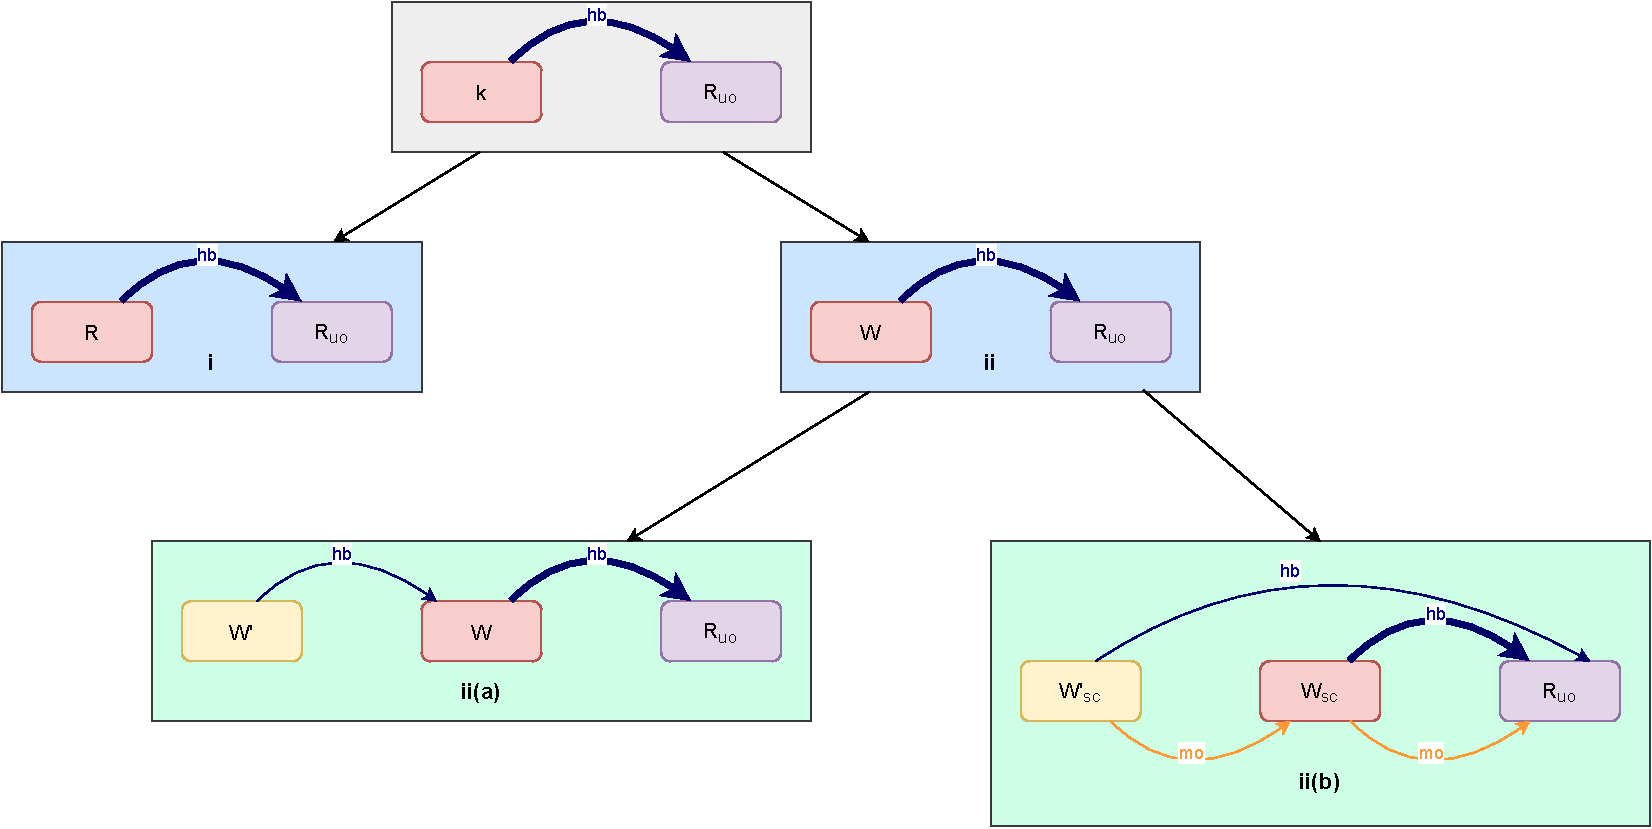
\includegraphics[scale=0.6]{5.InstructionReordering/4.ValidReorderingCandidate/ProofParts/Part4/part4(a).pdf}
        \caption{The impact of new relation $\reln{k}{hb}{e}$ where $\event{e}{R} \wedge \et{e}{uo}$ on observable behaviors.}
        \label{reord:case1}
    \end{figure}
    
    %Might have to elaborate this more
    \begin{itemize}
        
        \item For (i), when $k$ is a read, the pattern matches none of the Axioms.
        \item For (ii), when $k$ is a write, Axiom \ref{CoRe} (ii(a)) or Axiom \ref{SeqCsAt} (ii(b)) could restrict the read ($e$) from reading overlapping ranges of $W'$ with $W$.
    \end{itemize}
    
    Figure~\ref{reord:case2} shows a breakdown of sub-cases for case (b), varying based
    on the nature of event $k$.
    \begin{figure}[H]
        \centering
        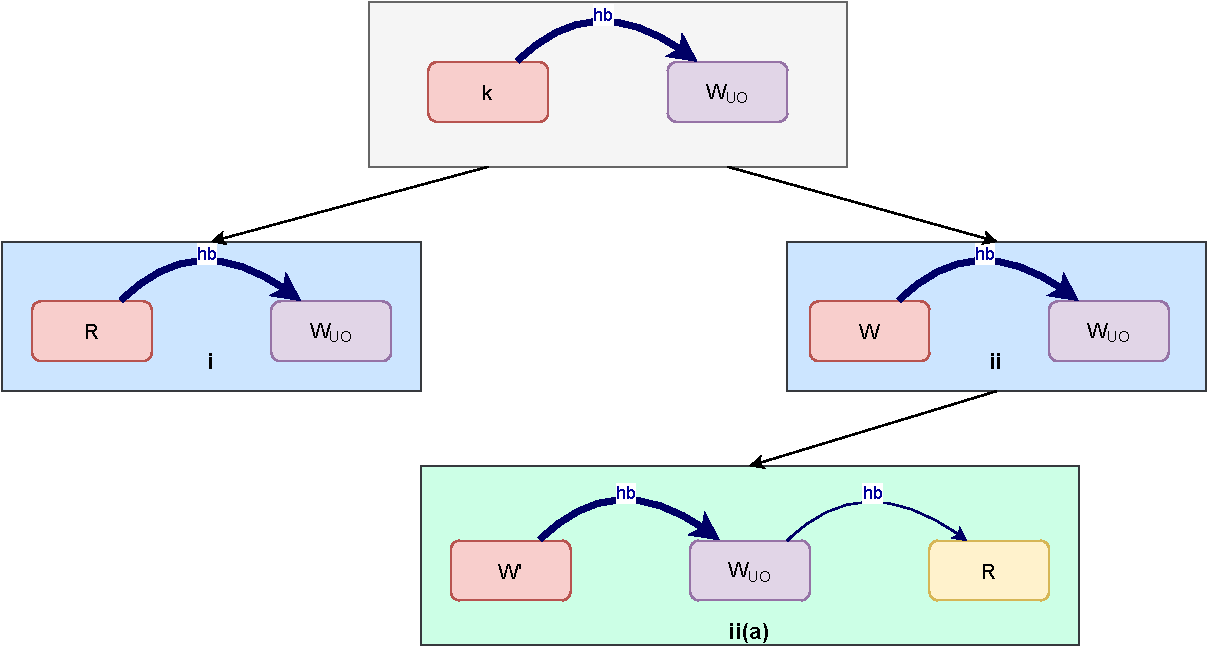
\includegraphics[scale=0.6]{5.InstructionReordering/4.ValidReorderingCandidate/ProofParts/Part4/part4(b).pdf}
        \caption{The impact of new relation $\reln{k}{hb}{e}$ where $\event{e}{W} \wedge \et{e}{uo}$ on observable behaviors.}
        \label{reord:case2}
    \end{figure}
          
    For case (b) we can observe the following from the above figure 
    \begin{itemize}
        \item For (i), when $k$ is a read, Axiom \ref{CoRe} restricts $k$ from reading from the write $e$. 
        \item For (ii), when $k$ is a write, Axiom \ref{CoRe} restricts some read from reading parts of $k$ due to the write $e$.   
    \end{itemize}

    Figure~\ref{reord:case3} shows a breakdown of sub-cases for case (c), varying based
    on the nature of event $k$.
    \begin{figure}[H]
        \centering
        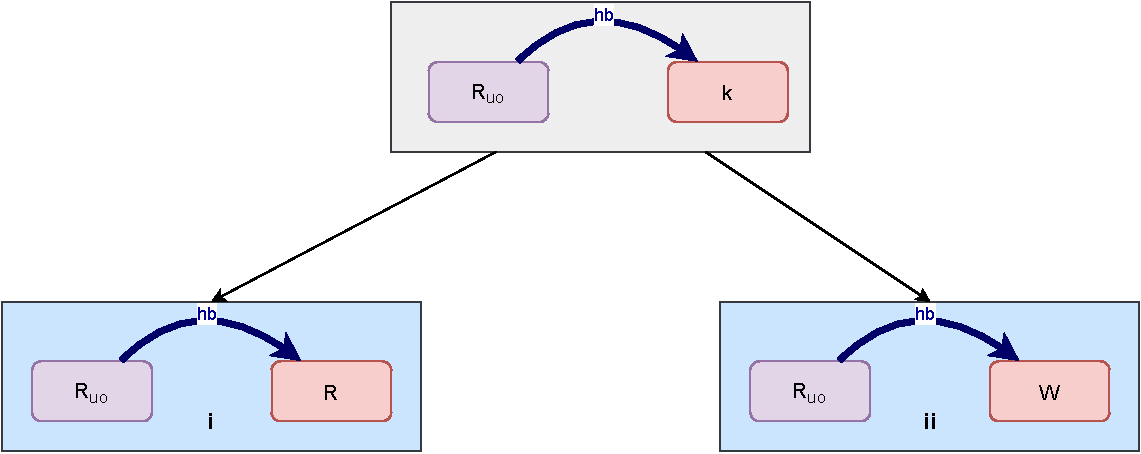
\includegraphics[scale=0.6]{5.InstructionReordering/4.ValidReorderingCandidate/ProofParts/Part4/part4(c).pdf}
        \caption{The impact of new relation $\reln{d}{hb}{k}$ where $\event{d}{R} \wedge \et{d}{uo}$ on observable behaviors.}
        \label{reord:case3}
    \end{figure}
    
    For case (c), we can observe the following from the above figure
    \begin{itemize}
        \item Case (i) does not correspond to any pattern restricted on the model, thus having no impact on the observable behaviors. 
        \item For (ii), when $k$ is a write, Axiom \ref{CoRe} restricts the read $d$ from reading values of write $k$. 
    \end{itemize}

    Figure~\ref{reord:case4} shows a breakdown of sub-cases for case (d), varying based
    on the nature of event $k$.
    \begin{figure}[H]
        \centering
        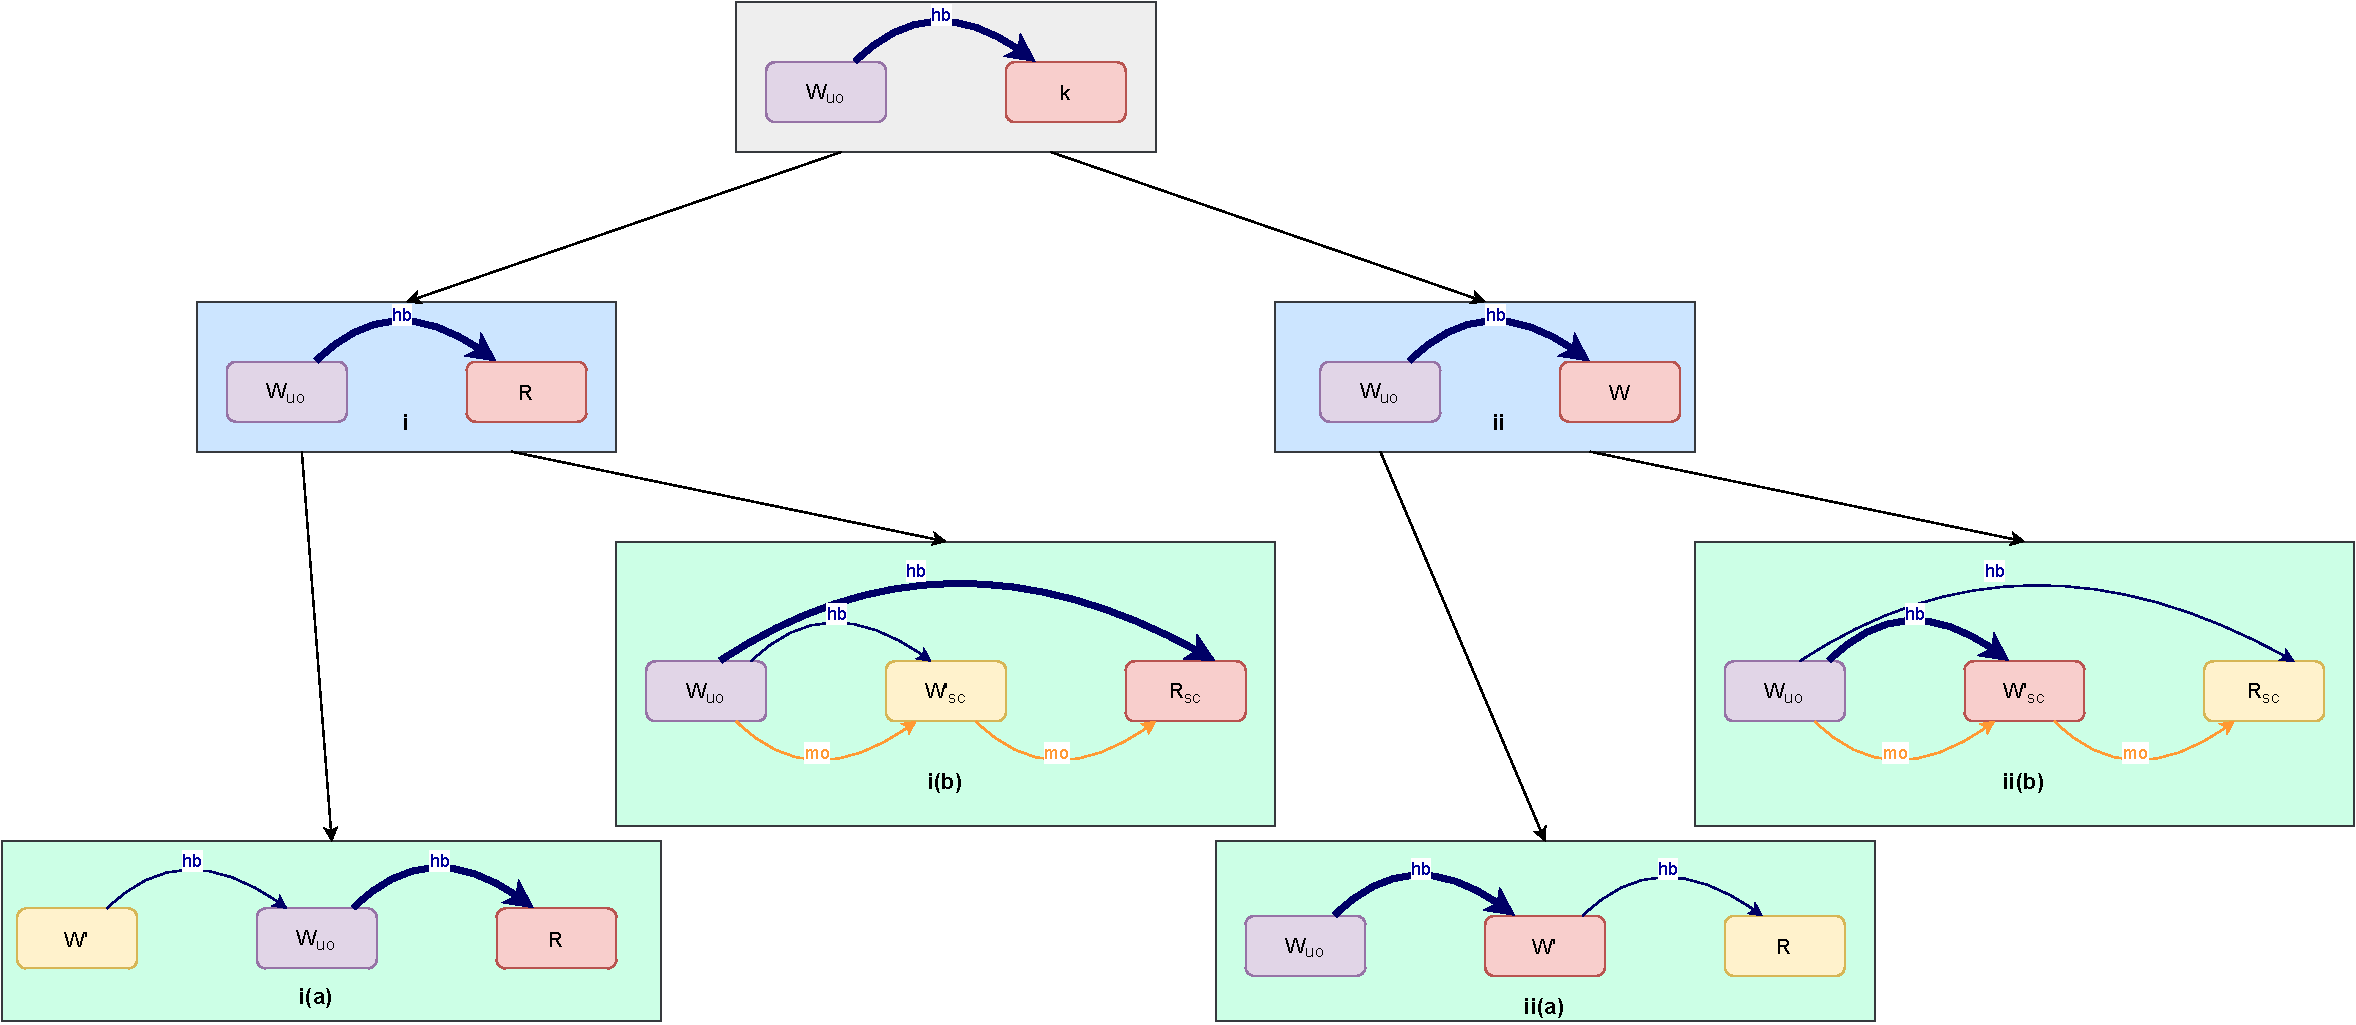
\includegraphics[scale=0.4]{5.InstructionReordering/4.ValidReorderingCandidate/ProofParts/Part4/part4(d).pdf}
        \caption{The impact of new relation $\reln{d}{hb}{k}$ where $\event{d}{W} \wedge \et{d}{uo}$ on observable behaviors.}
        \label{reord:case4}
    \end{figure}

    For case (d) we can observe the following 
    \begin{itemize}
        \item For case (i), Axiom \ref{CoRe} (i(a)) or Axiom \ref{SeqCsAt} (i(b)) could restrict a read $k$ from reading values of write $d$, 
        \item For case (ii), Axiom \ref{CoRe} (ii(a)) or Axiom \ref{SeqCsAt} (ii(b)) could restrict a read from reading values of write $d$, 
    \end{itemize}
  
    The above case wise analysis showed us that any new relation (apart from $\reln{d}{hb}{e}$), matching the patterns of the axioms, only enables in restricting possible observable behaviors, which are $\stck{_{rf}}$ relations. Thus, we can infer that no new observable behavior is introduced due to the new set of $\stck{_{hb}}$ relations. 
    
    In summary, Figure~\ref{reord:final_table} summarizes the valid cases where, we have a pair of valid pivots, where new relations do not introduce new observable behaviors and do not have cycles. 
    \begin{figure}[H]
        \centering
        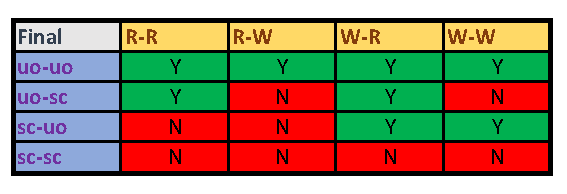
\includegraphics[scale=0.7]{5.InstructionReordering/4.ValidReorderingCandidate/part4_table.pdf}
        \caption{The final table summarizing the valid cases where observable behaviors will only be a subset after reordering.}
        \label{reord:final_table}
    \end{figure}
